\chapter{Relativistic Quantum Field Theory}
In non-relativistic quantum mechanics, the dispersion relation is
\begin{align*}
   E &= \frac{\pmb{p}^2}{2m}.
   \shortintertext{After promoting the momentum and energy into operators,}
   E &\mapsto i\hbar \frac{\partial}{\partial t}, \\
   \pmb{p} &\rightarrow -i\hbar \pmb{\nabla},
\end{align*}
we have the Schrödinger equation
\begin{align}
   i \frac{\partial}{\partial t} \psi(x,t) + \frac{1}{2m} \pmb{\nabla}^2 \psi(x,t) = 0.
\end{align}

Density of probability is defined via
\begin{align}
   \rho = |\psi|^2 = \psi \psi^*.
\end{align}
It obeys the continuity equation
\begin{align}
   -\frac{\partial}{\partial t } \int_V \rho \dd{V} &= \int \pmb{j} \cdot \pmb{n} \dd{S}, \notag\\
                                                    &= \int_V \pmb{\nabla} \cdot \pmb{j} \dd{V}, \notag \\
   \Rightarrow \frac{\partial \rho}{\partial t} + \div \pmb{j} &= 0.
\end{align}

Writing this explicitly
\begin{align}
   \frac{\partial \rho}{\partial t} &= \frac{\partial }{\partial t} \left( \psi \psi^* \right), \notag\\
                                    &= \psi \frac{\partial \psi^*}{\partial t} + \psi^* \frac{\partial \psi}{\partial t}, \notag \\
                                    &= \frac{i}{2m} \left( \psi^* \pmb{\nabla}^2 \psi -  \psi \pmb{\nabla}^2 \psi \right), \notag \\
   \Rightarrow \pmb{j} &= - \frac{i}{2m} \left( \psi^* \pmb{\nabla}^2 \psi -  \psi \pmb{\nabla}^2 \psi \right).
\end{align}

If we have a plane wave state, as an example 
\begin{align*}
   \psi &= N \euler^{i\pmb{p}\cdot \pmb{x} - i Et}, \\
   \pmb{j} &= \frac{\pmb{p}}{m} |N|^2.
\end{align*}

\section{Relativistic wave equation}
Now we enter the relativistic regime and the dispersion relation is
\begin{align*}
   E^2 &= \pmb{p}^2 + m^2.
   \shortintertext{Four-momentum is defined as before}
   p^\mu &= (E, \pmb{p}) \quad p_\mu = (E, -\pmb{p}), \\
   p^2 &= m^2.
\end{align*}

Promoting energy and momentum into operators,
\begin{align*}
   p^\mu &\mapsto i \partial^\mu, \\
   \partial_\mu \partial^\mu &= \frac{\partial ^2}{\partial^2 t} - \nabla^2.
\end{align*}
we have then Klein-Gordon (KG) equation
\begin{align}
   (\partial_\mu \partial^\mu + m^2) \phi(\pmb{x}, t) = 0.
\end{align}

The current in KG-theory is conserved as well
\begin{align}
   j^\mu &= (\rho, \pmb{j}) = i \left( \phi^* \partial^\mu \phi - \phi \partial^\mu \phi^* \right) \\
   \partial_\mu j^\mu &= 0
\end{align}

An example solution is 
\begin{align*}
   \phi = N \euler^{-ip\cdot x}, \\
   j^\mu = 2 p^\mu |N|^2.
\end{align*}

In terms of Lorentz transformation
\begin{align*}
   \rho \sim E.
\end{align*}

Energies of particles
\begin{align*}
   E^2 &= \pmb{p}^2 + m^2, \\
   E &= \pm \sqrt{\pmb{p}^2 + m^2}.
\end{align*}

It also implies negative probability
\begin{align*}
   E > 0 \mapsto \rho > 0, \\
   E < 0 \mapsto \rho < 0.
\end{align*}

\section{Feynman-Stückelberg Interpretation of negative energy states}
Current of "electron" with $E, \pmb{p}$ and charge $-e$ is
\begin{align*}
   j^\mu_{e^-} = 2e|N|^2(E,\pmb{p})
\end{align*}
Current of "positron" with $E, \pmb{p}$ and charge $+e$ is
\begin{align*}
   j^\mu_{e^+} = 2e|N|^2(E,\pmb{p})
   = - 2e|N|^2(-E,-\pmb{p})
\end{align*}

We can think of $E<0$ solution as particle flying backwards in time or $E > 0$ anti-particle forwards in time.
\begin{figure}[ht]
   \centering
   \includegraphics[width=0.8\linewidth]{fs-interpretation/fs-interpretation.eps}
   \caption{scattering process; horizontal time-axis; in the second diagram a electron positron pair is produced}%
   \label{fig:}
\end{figure}

In a relativistic systems we need to remember following points
\begin{itemize}
   \item anti-particles
   \item particle numbers are not conserved
\end{itemize}

\section{Electrodynamics (spin $1$)}
Maxwell equations are
\begin{align}
   \pmb{E} &= -\vec{\nabla} \phi - \frac{\dd}{\dd{t}}{\pmb{A}}, \\
   \pmb{B} &= \vec{\nabla} \times \pmb{A}, \\
   \vec{\nabla} \times \pmb{E} &= -\frac{\dd}{\dd{t}}{\pmb{B}}, \\
   \div \pmb{B} &= 0.
\end{align}

Field strength tensor and four-potential are
\begin{align}
   F_{\mu\nu} &= \partial_\mu A_\nu - \partial_\nu A_\mu, \\
   A^\mu(x) &= (\phi, \pmb{A}). \notag
\end{align}
The fields can be calculated from it
\begin{align}
   E^i &= F^{0i} = \partial^i A^0 - \partial ^0 A^i, \\
   B_i &= -\epsilon_{ijk} \partial^i A^k = -\epsilon_{0ijk}F^{jk}.
\end{align}

Often it is useful to use the dual tensor
\begin{align}
   \tilde{F}_{\mu\nu} &= \epsilon_{\mu\nu\sigma\tau} F^{\sigma \tau}.
   \shortintertext{The second set of maxwell equations is}
   \partial^{\mu} \tilde{F}_{\mu\nu} &= 0.
\end{align} 

The other set of two equations is 
\begin{align}
   \partial_\nu F^{\mu\nu} = 4\pi j^\mu.
\end{align}

$\pmb{E}, \pmb{B}$ are observable, $\pmb{A}$ is not. $A^\mu$ is not uniquely fixed by $\pmb{E}$ and $\pmb{B}$. It has the following gauge symmetry
\begin{align}
   \tilde{A}_{\mu} = A_\mu + \partial_\mu \Lambda(\pmb{x}, t).
\end{align}

Use this transformation to get the gauge conditions
\begin{align}
   \partial_\mu A^\mu = 0.
\end{align}

Plugging it back then we have the relativistic wave equation
\begin{align}
   \partial_\mu \partial^\mu A^\nu = 0.
\end{align}
it essentially is Klein-Gordon equation with mass $m=0$.

$A^\mu$ is a vector with spin $1$
\begin{align*}
   (j_+, j_-) = \left( \frac{1}{2}, \frac{1}{2} \right).
\end{align*}
It implied it has two transverse degrees of freedom. It has spin $1$ properties: $+1$, $0$, $-1$, in which $0$ mode does not exist.

\section{Description of Fermions}
Original motivation for Dirac is that he wants a linear equation in $E$ or $\frac{\partial}{\partial t}$
\begin{align*}
   p^\mu \mapsto i\partial^\mu
\end{align*}

Take the ansatz
\begin{align*}
   i\hbar \frac{\partial}{\partial t}\psi &= H \psi \\
   &= (\pmb{\alpha}\cdot \pmb{p} + \beta m ) \psi
\end{align*}
but $\pmb{\alpha}$ and $\beta$ unknown. It still has to obey the relativistic energy relation
\begin{align*}
   A &= \left( \alpha_ip_i + \beta m \right) \left( \alpha_ip_i + \beta m \right) \\
     &\stackrel{!}{=} \pmb{p}^2 + m^2 \\
     &= \alpha_i \alpha_j p_i p_j + \beta^2m^2 + \alpha_i \beta p_i m + \beta \alpha_j p_j m
\end{align*}

From this we demand
\begin{align}
   \beta^2 = 1 \\
   \alpha_i^2 = 1 \\
   \alpha_i \alpha_j + \alpha_j \alpha_i = 0 \\
   \alpha_i \beta + \beta \alpha_i = 0
\end{align}
So $\alpha$ and $\beta$ are not just numbers, but (can be proven to be) hermitian traceless matrices with eigenvalue $\pm 1$.  In addition, it only exits in even dimensions.
Since $\alpha_i$ and $\beta$ are $4\times4$ matrices. $\psi$ has to be a 4-component spinor.

For parity conservation need $(\frac{1}{2}, 0) \bigoplus (0, \frac{1}{2})$
Thus 
\begin{align*}
   \begin{pmatrix} \begin{pmatrix} & \\ & \end{pmatrix}_{2\times2} & \\ & \begin{pmatrix} & \\ &  \end{pmatrix}_{2\times2}   \end{pmatrix}
\end{align*}

There are different sets of $\alpha_i, \beta$ which satisfy the conditions. They are called representations.

Dirac-Pauli representation
\begin{align}
   \alpha_i &= \begin{pmatrix} 0 & \sigma^i \\ \sigma^i &  0 \end{pmatrix} \\
   \beta &= \begin{pmatrix} \id_2 & 0 \\ 0 & -\id_2\end{pmatrix}
\end{align}
with $\sigma^i$ the Pauli matrices.

Weyl (chiral) representation
\begin{align}
   \alpha^i &= \begin{pmatrix} -\sigma^i & 0 \\ 0 & \sigma^i \end{pmatrix}  \\
   \beta &= \begin{pmatrix} 0 & \id_2 \\ \id_2 & 0 \end{pmatrix}
\end{align}
they are mainly used in high energy physics (E $\gg m$).

\subsection{Gamma Matrices}
We now define 4 gamma matrices $\gamma^\mu$, $\mu=0,1,2,3$
\begin{align}
   \gamma^\mu = \left(\beta, \beta \pmb{\alpha} \right)
\end{align}
Note that having an index does not make it Lorentz vector.

The Clifford algebra is defined as following
\begin{align}
   \left\{ \gamma^\mu, \gamma^\nu \right\} = \gamma^\mu \gamma^\nu + \gamma^\nu \gamma^\mu = 2 g^{\mu\nu}
\end{align}

In Dirac-Pauli representation
\begin{align}
   \gamma^0 &= \begin{pmatrix} \id & 0 \\ 0 & -\id \end{pmatrix} \\
   \gamma^i &= \begin{pmatrix} 0 & \sigma^i \\ -\sigma^i & 0 \end{pmatrix} \\
   \gamma^5 &= i \gamma^0 \gamma^1 \gamma^2 \gamma^3 = \begin{pmatrix} 0 & \id \\ \id & 0\end{pmatrix}
\end{align}

In Weyl representation 
\begin{align*}
   \gamma^0 \leftrightarrow \gamma^5
\end{align*}

Rewriting the Dirac equation using $\gamma$s
\begin{align}
   i \partial_t \psi &= \left( \pmb{\alpha} \cdot \pmb{p} + \beta m  \right) \psi \notag\\
   i \partial_t \psi &= -i \pmb{\alpha} \cdot \vec{\nabla} \psi + m \beta \psi \notag\\
   i \beta \partial_t \psi &= -i \beta \pmb{\alpha} \cdot \vec{\nabla} \psi + m \psi \notag\\
   \left(i\gamma^\mu \partial_\mu - m \right) \psi &= 0
\end{align}
Conventionally we use $\phi$ for spin $0$ particle and $A_\mu$ for spin $1$.

It is convenient to also have an equation for $\psi^\dagger$. First one can show $\gamma^{\dagger\mu} = \gamma^0 \gamma^\mu \gamma^0$.
\begin{itemize}
   \item $\mu = 0$: $\gamma^0 = \beta$ and $\gamma^{\dagger\, 0} = \gamma^0 \gamma^0 \gamma^0$ $\Rightarrow \beta^2 = \id_4$
   \item $\gamma^{\dagger\mu} = (\beta \alpha^k)^\dagger = (\alpha^k)^\dagger \beta^\dagger = \alpha^k \beta = \beta^2 \alpha^k \beta = \beta \gamma^k \beta = \gamma^0 \gamma^k \gamma^0$
\end{itemize}

\begin{align}
   i \gamma^0 \partial_0 \psi + i \gamma^k \partial_k \partial - m \psi = 0 \notag\\
   -i \partial_0 \psi^\dagger (\gamma^0)^\dagger - i(\partial_k \psi^\dagger) \gamma^{\dagger\; k} - m \psi^\dagger = 0 \notag \\
   -i \partial_0 \psi^\dagger \gamma^0 - i(\partial_k \psi^\dagger) \gamma^0 \gamma^k \gamma^0 - m \psi^\dagger = 0 \notag \\
   \shortintertext{define $\bar{\psi} = \psi^\dagger \gamma^0$}
   -i \partial_0 \bar{\psi} \gamma^0 - i \partial_\mu \bar{\psi} \gamma^\mu - m \bar{\psi} = 0 \notag \\
   i(\partial_\mu \bar{\psi}) \gamma^\mu + m \bar{\psi} = 0
\end{align}

\subsection{Free Particle Solution to Dirac Equation}
\begin{align*}
   \left( i \gamma^\mu \partial_\mu - m \right) \psi &= 0 \\
   \shortintertext{multiplying $\gamma^\nu \partial_\nu$ from left}
   i\gamma^\mu \gamma^\nu \partial_\mu \partial_\nu \psi - m \gamma^\nu \partial_\nu \psi &= 0 \\
   i \gamma^\mu \gamma^\nu \partial_\mu \partial_\nu \psi + i m^2 \psi &= 0 \\
\end{align*}

\begin{align*}
   \gamma^\mu \gamma^\nu  &= \frac{1}{2} \left( \gamma^\mu \gamma^\nu + \gamma^\nu \gamma^\mu  \right) \\
                          &= \frac{1}{2} \left( \gamma^\mu \gamma^\nu - \gamma^\nu \gamma^\mu + 2g^{\mu\nu} \right) \\
                          &= \frac{1}{2} \left[ \gamma^\mu , \gamma^\nu \right] + g^{\mu\nu}
\end{align*}
The commutator is anti-symmetric and multiplying to symmetric tensor (derivatives) the term must vanish.

Each component of spinor satisfies the Klein-Gordon equation.
\begin{align}
   (\partial_\mu \partial^\mu + m^2) \psi_i = 0
\end{align}

Thus we can write the solution as plane-wave
\begin{align}
   \psi = u(\pmb{p}) \euler^{-ipx}
\end{align}
$u(\pmb{p})$ is also a 4-component object but as function $\pmb{p}$ not $\pmb{x}$

Insert back into Dirac equation, then we have Dirac equation in momentum space
\begin{align}
   \left( \gamma^\mu p_\mu - m \right) u(\pmb{p}) = 0
\end{align}

Solution by considering Dirac-Pauli representation
\begin{align*}
   \left( \slashed{p} - m \right) u(\pmb{p}) = \begin{pmatrix} (E-m) \id & - \pmb{p} \cdot \pmb{\sigma} \\ \pmb{p} \cdot \pmb{\sigma} & -(E+m) \id \end{pmatrix} 
   \begin{pmatrix} u_A \\ u_B\end{pmatrix}
\end{align*}

$\pmb{p} = 0$ then $E = \pm m$

\begin{itemize}
   \item $E = +m$ Two solutions 
      \begin{align*}
         u_B = \begin{pmatrix} 1 \\ 0 \end{pmatrix} , \begin{pmatrix} 0 \\ 1\end{pmatrix}
      \end{align*}

   \item $E=-m$
      \begin{align*}
         u_A = \begin{pmatrix} 1 \\ 0\end{pmatrix}, \begin{pmatrix} 0 \\ 1\end{pmatrix}
      \end{align*}
\end{itemize}

$\pmb{p} = 0$
\begin{align}
   \pmb{\sigma} \cdot \pmb{p} u_B &= (E-m) u_A \\
   \pmb{\sigma} \cdot \pmb{p} u_A &= (E+m) u_B
\end{align}

\begin{itemize}
   \item $E>0$ 
      \begin{align*}
         \chi^{(1)} &= \begin{pmatrix} 1 \\ 0\end{pmatrix} \\
         \chi^{(2)} &= \begin{pmatrix} 0 \\ 1\end{pmatrix}
      \end{align*}
\end{itemize}

Ansatz $u_A^{(s)} = \chi^{(s)}$
\begin{align}
   u_B^{(s)} = \frac{\pmb{\sigma}\cdot\pmb{p}}{E + m} &\quad u_A^{(s)} = \frac{\pmb{\sigma}\cdot\pmb{p}}{E + m} \chi^{(s)} \notag\\
   u(\pmb{p}) &= N \begin{pmatrix} \chi^{(s)} \\ \frac{\pmb{\sigma}\cdot\pmb{p}}{E + m} \chi^{(s)}\end{pmatrix}
\end{align}

$E < 0$ and $u_B^{(s)} = \chi^{(s)}$
\begin{align}
   u(\pmb{p}) = N \begin{pmatrix} -\frac{\pmb{\sigma}\cdot\pmb{p}}{E + m} \chi^{(s)} \\ \chi^{(s)}\end{pmatrix}
\end{align}

One can show $u^{\dagger (r)} u^{(s)} = N^2 \delta^{rs}$

Two fold degeneracy in each case. $ \begin{pmatrix} 1 \\ 0\end{pmatrix}$ and $ \begin{pmatrix} 0 \\ 1\end{pmatrix} $ for $E > 0$ and $E < 0$. There must be another observable which commutes with $H$ and $\pmb{p}$.
\begin{align*}
   H = \gamma^i p_i + \gamma^0 m
\end{align*}
\begin{align}
   \pmb{S} \cdot \hat{P} = \frac{1}{2} \begin{pmatrix} \pmb{\sigma}\cdot\pmb{p} & 0 \\ 0 & \pmb{\sigma}\cdot \hat{p}\end{pmatrix}
\end{align}

Helicity
\begin{align}
   \frac{1}{2} \pmb{\sigma} \cdot {\hat{p}} &= \frac{1}{2} \begin{pmatrix} \hat{p}_z & \hat{p}_x + i\hat{p}_y \\ \hat{p}_x -i \hat{p}_y & -\hat{p}_z\end{pmatrix} \\
   \det(\pmb{\sigma} \cdot \hat{p}) &= - \hat{p}^2 = - 1
\end{align}
  
Determinant is the product of two eigenvalues, then
\begin{align*}
   \lambda_1 + \lambda_2 &= 0 \\
   \lambda_1 \cdot \lambda_2 &= 1 \\
   \lambda_{1,2} &= \pm 1
\end{align*}

Antiparticle solution $u^{(3,4)}(-\pmb{p}) e^{-i(-p)x} = v^{(2,1)}$
\begin{align}
   \left( \slashed{p} + m \right)v(\pmb{p}) = 0
\end{align}

Normalization is
\begin{align}
   \int \rho \dd{V} = 2E \\
   N = \sqrt{E+m}
\end{align}

Completeness relation (spin sums)
\begin{align}
   \sum u^{(s)}(p) \bar{u}^{(s)}(p ) = \left( \slashed{p} + m \right) \\
   \sum v^{(s)}(p) \bar{v}^{(s)}(p ) = \left( \slashed{p} - m \right)
\end{align}

Define a projector projecting out positive and negative energy states
\begin{align}
   \Lambda_{\pm} = \frac{\pm \slashed{p} + m}{2m}
\end{align}

In Chiral (Weyl) representation
\begin{align}
   \left( \slashed{p} - m \right) u(\pmb{p}) = \begin{pmatrix} m & p \cdot \sigma \\ \vecp \cdot \bar{\sigma} & -m \end{pmatrix} \begin{pmatrix} u_L \\ u_R\end{pmatrix}
\end{align}
$\bar{\sigma} = (\sigma^0 , -\pmb{\sigma})$ and $\sigma^0 = \id_2$

Weyl equation
\begin{align}
   \begin{split}
    -m u_L + p\cdot \sigma u_R = 0 \\
   p \cdot \bar{\sigma} u_L - m u_R = 0
   \end{split}
\end{align}
if $m=0$, the equations decouple from each other.

%%%%%%%%%%%%%%%%%%%%%%%%%%%%%%%%%%%%%%%%%%%%%%%%%%%%%%%%%%%%%%%
% Lecture on 21.10
%%%%%%%%%%%%%%%%%%%%%%%%%%%%%%%%%%%%%%%%%%%%%%%%%%%%%%%%%%%%%%%

We want to construct Lagrangians involving the fields $\psi$, $A_\mu$ and $\psi$. The reason we choose Lagrangians as opposed to Hamiltonians, is that Hamiltonian $H$ is associated with energy of system, which is not Lorentz (or relativistic) invariant. But Lagrangian density is $S = \int \dd{t} = \int \dd[4]{x} \lag$. In natural unit, the action is dimensionless. One can in addition prove $\dd[4]{x}$ is Lorentz invariant.  The fact that $\lag$ is Lorentz invariant, means that $\lag$ need to have at least $2$ spin-$\frac{1}{2}$ fields $\psi$ or $\bar{\psi}$, to make a spin-$0$.

We are interested in the objects like
\begin{align*}
   \bar{\psi}(\gamma^\mu) \psi
\end{align*}

Representation of the Lorentz group can be split into $ \left( \frac{1}{2}, 0 \right)$ and $ \left( 0, \frac{1}{2} \right)$. In Weyl or chiral representation, $\psi_L$ has $ \left( \frac{1}{2}, 0 \right)$ and $\psi_R$ $ \left( 0, \frac{1}{2} \right)$.

Here we are taking a different approach from the paper \cite{Dreiner_2010}. First define
\begin{align}
   \sigma^{\mu\nu} = \frac{i}{2} \left[ \gamma^\mu, \gamma^\nu \right]
\end{align}

We want to find out the transformation of $\psi = u(\pmb{p})e^{-ip\cdot x}$. Note that the second factor is written in covariant form, i.e.~Lorentz invairant. Consider the Dirac equation in two different frames $x' = \Lambda x$
\begin{align}
   i \gamma^\mu \frac{\partial \psi(x)}{\partial x^\mu} - m \psi(x) = 0 \label{math:dirac}\\
   i \gamma^\mu \frac{\partial \psi'(x')}{\partial x'^\mu} - m \psi'(x') = 0 \label{math:diracP}
\end{align}

We make the ansatz that the spinor transforms with $S$ 
\begin{align}
   \psi'(x') = S\psi(x) \label{math:psiS}
\end{align}
$S$ must be independent of $x$. Plug \ref{math:psiS} into \ref{math:diracP} 
\begin{align*}
   i \gamma^\mu \frac{\partial}{\partial x'^\mu} \left[ S \psi(x) \right] - m S \psi(x) &= 0 \\
   i S^{-1} \gamma^\mu S \frac{\partial \psi (x)}{\partial x^\nu} \underbrace{\frac{\partial x^\nu}{\partial x'^\mu}}_{=\Lambda^{-1}} - m\psi(x)  &= 0
\end{align*}

This equation must be the same as \ref{math:dirac}, then we get
\begin{align}
   S^{-1} \gamma^\mu S \left[ \Lambda^{-1} \right]^\nu_{\; \mu} &= \gamma^\nu \notag\\
   S^{-1} \gamma^\mu S &= \Lambda^\mu_{\; \nu} \gamma^\nu
\end{align}

$S_{\mu\nu}$ is anti-symmetric in $\mu$ and $\nu$
\begin{align}
   S_i &= \frac{1}{2} \epsilon_{ijk} S^{jk} \\
   K_i &= S^{0i} \\
   \psi'_\alpha(x') &= \left[\exp(-\frac{i}{2} \Theta^{\mu\nu} S_{\mu\nu})\right]^\beta_\alpha \psi_\beta \\
   \omega_i &= \frac{1}{2} \epsilon_{ijk} \Theta_{ijk}
\end{align}

Lorentz transformation containing rotations and boosts, but infinitesimal version (infinitesimally different from $\id$)
\begin{align}
   \Lambda^\nu_{\; \mu} = \delta^\nu_{\;\mu} + \epsilon^\nu_{\;\mu}
\end{align}

We will show in the exercise the expression of transformation under boosts and rotations
\begin{align}
   S_L &= \id_4 - \frac{i}{4} \sigma_{\mu\nu} \epsilon^{\mu\nu} \\
   S_L^{-1} &= \id_4 + \frac{i}{4} \sigma_{\mu\nu} \epsilon^{\mu\nu}
\end{align}

It satisfies $S^{-1} \gamma^\mu S = \Lambda^{\mu}_{\;\nu} \gamma^\nu = \gamma^\nu + \epsilon^\mu_{\;\nu} \gamma^\nu$
\begin{align*}
   \left(\id_4 + \frac{i}{4} \sigma_{\mu\nu} \epsilon^{\mu\nu} \right) \gamma^\mu \left(\id_4 - \frac{i}{4} \sigma_{\mu\nu} \epsilon^{\mu\nu}\right)
   &= \gamma^\mu + \frac{i}{4} \left[ \sigma_{\alpha\beta} \gamma^\mu - \gamma^\mu \sigma_{\alpha\beta} \right]\epsilon^{\alpha \beta} 
   \shortintertext{somehow}
   &= \gamma^\mu + \epsilon^\mu_{\; \nu} \gamma^\nu
\end{align*}

Parity transformation cannot be written in infinitesimal form. Thus it is often called (one of) discrete transformation.
\begin{align}
\Lambda_{\text{P}} = \diag(+1,-1,-1,-1)
\end{align}
Parity symmetry is naturally violated. Especially in weak interaction, since neutrinos are left-handed $\nu_L$.
\begin{align}
   S^{-1}_\text{P} \gamma^\mu S_\text{P} = \Lambda^\mu_{\text{P}\, \nu} \gamma^\nu
\end{align}

\begin{itemize}
   \item For $\mu = 0$ 
      \begin{align*}
S^{-1}_\text{P} \gamma^0 S_\text{P} = \gamma^0
      \end{align*}
   \item For $\mu=i$
      \begin{align*}
S^{-1}_\text{P} \gamma^i S_\text{P} = -\gamma^i
      \end{align*}
\end{itemize}

It is easy to show $S_\text{P} = \gamma^0$ satisfies the equations. Then the spinor transform under parity like
\begin{align}
   \psi'(t, -\pmb{x}) = \gamma^0 \psi(t,\pmb{x})
\end{align}

In Dirac-Pauli representation $\gamma^0 = \begin{pmatrix} \id_2 & 0 \\ 0 & \id_2 \end{pmatrix}$
\begin{align*}
   \psi = \begin{pmatrix} \psi_1 \\ \psi_2 \\ \psi_3 \\ \psi_4 \end{pmatrix} \quad
   \psi' = \begin{pmatrix} \psi_1 \\ \psi_2 \\ -\psi_3 \\ -\psi_4 \end{pmatrix} 
\end{align*}

In chiral representation $\gamma^0 = \begin{pmatrix} 0 & \id_2 \\ \id_2 & 0 \end{pmatrix}$ and 
\begin{align*}
\psi = \begin{pmatrix} \psi_L \\ \psi_R\end{pmatrix} \quad
\psi' = \begin{pmatrix} \psi_R \\ \psi_L \end{pmatrix}
\end{align*}

Recall $\bar{\psi} = \psi^\dagger \gamma^0$. 
\begin{align*}
   \bar{\psi}' &= \psi'^\dagger \gamma^0 = \psi^\dagger S^\dagger \gamma^0 \\
   \shortintertext{it can easily be shown using the explicit expresseion of $S_L$ and $S_L$. Parity transformation is $\gamma^0$.}
               &= \psi^\dagger \gamma^0 S^{-1} \\
               &= \bar{\psi} S^{-1}
\end{align*}

There are $16$ different bilinear $\bar{\psi} A \psi$
\begin{itemize}
   \item $A = \id_4$
      \begin{align*}
      \bar{\psi}' \psi' = (\bar{\psi} S^{-1}) (S \psi) = \bar{\psi} \psi
      \end{align*}
   \item $A = \gamma^\mu$
      \begin{align*}
          \bar{\psi}' \gamma^\mu \psi' = \bar{\psi} S^{-1} \gamma^\mu S \psi = \Lambda^\mu_{\;\nu} \left( \bar{\psi} \gamma^\nu \psi \right)
      \end{align*}
      It transforms exactly like a Lorentz vector. Especially under parity
      \begin{align*}
         \bar{\psi}' \gamma^\mu \psi' = \begin{cases}
            \bar{\psi}' \gamma^0 \psi'  & \mu = 0 \\
            -\bar{\psi}' \gamma^i \psi'   & \mu = 1,2,3
         \end{cases}
      \end{align*}
   \item $A = \gamma^5$
      \begin{align*}
         \bar{\psi}' \gamma^5 \psi' &= \bar{\psi} S_L^{-1} \gamma^5 S_L \psi 
          \shortintertext{$ \left\{ \gamma^\mu, \gamma^5 \right\} = 0$ and  $\sigma_{\mu\nu}$ contains two $\gamma$s}
                                    &= \bar{\psi} \gamma^5 \psi 
      \end{align*}
      It is a scalar under boosts and rotations.
      Under parity it is pseudoscalar, like pions.
      \begin{align*}
         \gamma^5 S_\text{P} = \gamma^5 \gamma^0 = - S_\text{P} \gamma^5
         \shortintertext{thus}
            \bar{\psi}' \gamma^5 \psi' = - \bar{\psi}' \gamma^5 \psi'
      \end{align*}

      For experiments, look it up in Introduction to HEP, Perkins
\end{itemize}

Chiral spinors (in chiral representation)
\begin{align}
   P_R &= \frac{1}{2} \left( \id_4 + \gamma^5 \right) = \begin{pmatrix} 0&0\\0&\id_2\end{pmatrix} \\
   P_L &= \frac{1}{2} \left( \id_4 - \gamma^5 \right) = \begin{pmatrix} \id_2&0\\0&0\end{pmatrix}
\end{align}

If $\psi$ written like $\psi = \begin{pmatrix} \chi_L \\ \chi_R \end{pmatrix}$, it is in chiral representation
\begin{align*}
   P_L \psi &= \begin{pmatrix} \chi_L \\ 0\end{pmatrix} = \psi_L \\
   P_R \psi &= \begin{pmatrix} 0 \\ \chi_R \end{pmatrix} = \psi_R
\end{align*}

They are projectors
\begin{align*}
   P_R^2 &= \frac{1}{4} (\id_4 + \gamma^5) (\id_4 + \gamma^5) = \frac{1}{4} (\id_4 + 2 \gamma^5 + (\gamma^5)^2) = P_R \\
   P_L^2 &= P_L
\end{align*}

They also project onto complete space meaning $P_L + P_R = \id_4$.

Left-handed particles have spin and momentum in the opposite direction and right-handed in the same direction. In Dirac-Pauli representation in high energy limit
\begin{align*}
   \gamma^5 u^{(5)} \approx \begin{pmatrix} \pmb{\sigma} \cdot \hat{p} & 0 \\ 0 & \pmb{\sigma} \cdot \hat{p}\end{pmatrix}
\end{align*}

To show this take the free particle solution ($E>0$)
\begin{align*}
   u^{(s)} &= N \begin{pmatrix} \chi^{(s)} \\ \frac{\pmb{\sigma \cdot \pmb{p}}}{E+m} \chi^{(s)}\end{pmatrix} \\
   \gamma^5 u^{(s)} &= N  \begin{pmatrix}  \frac{\pmb{\sigma \cdot \pmb{p}}}{E+m} \chi^{(s)} \\ \chi^{(s)}  \end{pmatrix} \approx N \begin{pmatrix} \pmb{\sigma} \cdot \hat{p} \chi^{(s)} \\ \chi^{(s)} \end{pmatrix} \\
   \shortintertext{In general $(\pmb{\sigma \cdot \pmb{a}})^2 = \pmb{a}^2 \id$} 
   &=  N \pmb{\sigma} \cdot \hat{p} \begin{pmatrix} \chi^{(s)} \\ \pmb{\sigma} \cdot \hat{p} \chi^{(s)} \end{pmatrix}  = \underbrace{\pmb{\sigma} \cdot \hat{p}}_{\text{helicity operator}} u^{(s)} \\
\end{align*}

At high energy limit ($E \gg m$), $\gamma^5$ helicity operator, but not at low energy. Chirality $\psi_{L,R}$ is always a good quantum number.

%%%%%%%%%%%%%%%%%%%%%%%%%%%%%%%%%%%%%%%%%%%%%%%%%%%%%%%%%%%%%%%%%%%%%%
% Lecture on 22.10 
%%%%%%%%%%%%%%%%%%%%%%%%%%%%%%%%%%%%%%%%%%%%%%%%%%%%%%%%%%%%%%%%%%%%%

\paragraph{Angular momentum}
Must be another observable which commutes with $H$ and $P$ (u = u(\pmb{p}))
\begin{align}
   \pmb{\Sigma} \cdot \hat{p} &= \begin{pmatrix} \pmb{\sigma} \cdot \hat{p} & 0 \\ 0 &\pmb{\sigma} \cdot \hat{p} \end{pmatrix} \\
   H &= \alpha \cdot P + \beta m \\
   \left[ H, \pmb{\Sigma} \cdot \hat{p} \right] &= 0
\end{align}

Angular momentum operator is defined as 
\begin{align}
   \pmb{L} = \pmb{r} \times \pmb{P} \\
\end{align}

Use the relation $\left[ \hat{x}_i, \hat{P}_j \right] = i \delta_{ij}$ and check the commutation
\begin{align*}
   \left[ H, L_1 \right] &= \left[ \pmb{\alpha} \cdot \pmb{P}, x_2 P_3 - x_3 P_2 \right] \\
                         &= \left[ \alpha_1 P_1 + \alpha_2 P_2 + \alpha_3 P_3, x_2 P_3  - x_3 P_2 \right] \\
                         &= \alpha_2 \left[ P_2, x_2 \right] P_3 - \alpha_3 \left[ P_3, x_3 \right] P_2  \\
                         &= -i \left( \alpha_2 P_3 - \alpha_3 P_2 \right)\\
                         &= -i (\alpha \times P)_1
\end{align*}
Thus $ \left[ H, \pmb{L} \right] = -i (\pmb{\alpha} \times P) \neq 0$. In other word, $L$ not conserved.

But we observe
\begin{align}
   \pmb{\Sigma} &= \begin{pmatrix} \pmb{\sigma} & 0 \\ 0 & \pmb{\sigma}\end{pmatrix} \\
   \left[ H, \pmb{\Sigma} \right] &= 2i(\pmb{\alpha} \times P)
\end{align}
Thus define total angular momentum, second term describe the intrinsic angular momentum of particles
\begin{align}
   \pmb{J} = \pmb{L} + \frac{1}{2} \pmb{\Sigma}
\end{align}
and $J$ is conserved.

\paragraph{Charge conjugation}
Equation describing fermions couple to electromagnetic current
\begin{align}
   \left[ \gamma^\mu \left( i \partial_\mu + e A_\mu \right) - m \right] \psi = 0 \label{math:diracEM}
\end{align}
with $e$ the electric charge of electron and $A_\mu(x)$ vector potential in electromagnetism.
 
For positron the charge is the opposite
\begin{align}
   \left[ \gamma^\mu \left( i \partial_\mu - e A_\mu \right) - m \right] \psi^\text{C} = 0 \label{math:diracEMP}
\end{align}
$\psi^{\text{C}}$ is the charge conjugate of  $\psi$. We want to know the relation between $\psi \leftrightarrow \psi^{\text{C}}$. Take complex conjugate of equation \ref{math:diracEM}
\begin{align}
   \left[ -(\gamma^{\mu})^{*} \left( i \partial_\mu - eA_\mu \right) - m \right] \psi^* &= 0 \label{math:diracEMCC}
   \shortintertext{We postulate a matrix $C$ so that $\psi^\text{C} = C\gamma^0 \psi^*$ and multiply equation \ref{math:diracEMCC} by $C \gamma^0$ from left. }
   C \gamma^0 \left[ -\left(\gamma^{\mu}\right)^* \left( i \partial_\mu - eA_\mu \right) - m \right] \psi^* &= 0 \notag \\
   \shortintertext{It must be the same as equation \ref{math:diracEMP}. Thus}
   - (C \gamma^0) (\gamma^{\mu})^{*} &= \gamma^\mu C \gamma^0 \notag \\
   - C (\gamma^{\mu})^{\text{T}} &= \gamma^\mu C \notag \\
   C \gamma^{\mu T} C^{-1} &= - \gamma^\mu \notag \\
   C &= i \gamma^0 \gamma^2
\end{align}

Then we find
\begin{align}
   \psi^{\text{C}} = C \gamma^0 \psi^* = C \bar{\psi}^\text{T}
\end{align}

It would be interesting to compare $P_L (\psi^\text{C})$ and $(P_L \psi)^\text{C}$

\paragraph{Continuity equation for $\psi$}
\begin{align}
   \rho = \psi^\dagger \psi = \bar{\psi} \gamma^0 \psi
\end{align}
Multiply $\bar{\psi}$ from left to dirac equation and $\psi$ from right to conjugated Dirac equation
\begin{align*}
   \bar{\psi} \left( i \gamma^\mu \partial_\mu - m \right) \psi = 0, &\qquad i (\partial_\mu \bar{\psi}) \gamma^\mu \psi + m \bar{\psi} \psi = 0\\
   \bar\psi \gamma^\mu (\partial_\mu \psi) + (\partial_\mu \bar\psi) \gamma^\mu \psi &= 0 \\
   \partial_\mu ( \bar{\psi} \gamma^\mu \psi) &= 0 \\
   \partial_\mu j^\mu &= 0
\end{align*}

\section{Classical Field Theory} 
\paragraph{Reminder} 
\begin{align*}
   \shortintertext{Lagrangian and action}
   L = L (q_i, \dot{q}_i, t) &\qquad   S = \int \dd{t} L \\
   \shortintertext{Variantion principle}
   \delta S &= 0 \\
   \shortintertext{is equivalent to Euler-Lagrange equations}
   \frac{\dd}{\dd{t}} \frac{\partial L}{ \partial \dot{q}_i}& =\frac{\partial L}{\partial q_i}
\end{align*} 

Going to field theory, we transform $q(t) \rightarrow \phi(x)$ and $L \rightarrow \lag$
\begin{align*}
   \lag &= \lag \left(\phi, \frac{\partial \phi}{\partial x^\mu}, x_\mu \right) \\
   S &= \int \dd[4]{x} \lag(\phi, \frac{\partial \phi}{\partial x^\mu}, x_\mu) 
\end{align*}

Using the variation principle
\begin{align*}
   \delta S &= \sum_i \frac{\dd{S}}{\dd{\alpha_i}} \delta \alpha_i \\
            &= \sum_i \int \dd[4]{x} \left\{ \frac{\partial \lag}{\partial \phi} \frac{\partial \phi}{\partial \alpha_i} \delta \alpha_i + \frac{\partial \lag}{\partial (\partial_\mu \phi)} \frac{\partial (\partial_\mu \phi)}{\partial \alpha_i} \delta \alpha_i \right\} \\
            &= \sum_i \int \dd[4]{x} \left\{ \frac{\partial \lag}{\partial \phi} \frac{\partial \phi}{\partial \alpha_i} - \left( \partial_\mu \frac{\partial \lag}{\partial (\partial_\mu \phi)} \frac{\partial \phi}{\partial \alpha_i} \right) \right\}\delta \alpha_i + \eval{\frac{\partial \lag}{\partial (\partial_\mu \phi)} \frac{\partial \phi}{\partial \alpha_i} \delta\alpha_i}_{x_0}^{x_1}
\end{align*}

Then we have our new Euler-Lagrange equations for continuous fields
\begin{align}
   \frac{\partial \lag}{\partial \phi} - \partial_\mu \frac{\partial \lag}{\partial(\partial_\mu \phi)} = 0
\end{align}

\paragraph{Conservation Laws and Noether Theorem}
Reminder: Under transformation $t \mapsto t' = t + \delta b$, system stays invariant if $\delta_T L = \frac{\dd}{\dd{t}}(\delta \Omega)$.

$\delta \Omega = 0$ if $L$ invariant

\begin{align*}
   \delta_T L = L(q, \dot{q}, t+\delta b) - L (q, \dot{q}, t) = \frac{\partial L}{\partial t} \delta b
\end{align*}

\begin{align*}
   \frac{\dd{L}}{\dd{t}} &= \frac{\partial L}{\partial t} + \frac{\partial L}{\partial q} \dot{q} + \frac{\partial L}{\partial \dot{q}} \ddot{q} \\
                         &= \frac{\partial L}{\partial t} + \frac{\dd}{\dd{t}} \left (\frac{\partial L}{\partial \dot{q}} \right) \dot{q} + \frac{\partial L}{\partial \dot{q}} \ddot{q} \\
                         &= \frac{\partial L}{\partial t} + \frac{\dd}{\dd{t}} \left[ \frac{\partial L}{\partial \dot{q}} \dot{q} \right] \\
\end{align*}

System invariant if
\begin{align}
   \frac{\partial L}{\partial t} = \frac{\dd}{\dd{t} } (\delta \Omega)
\end{align}
if $L$ not dependent explicitly on $t$, $\dd{L} / \dd{t} = 0$

If $\partial L / \partial t = 0$, the conserved quantity
\begin{align*}
   \frac{\dd}{\dd{t}} \left[ L - \frac{\partial L}{\partial \dot{q}} \dot{q} \right] &= 0 \\
   L - \frac{\partial L}{\partial \dot{q}} \dot{q} &= -H = L - \dot{q} p
\end{align*}
using legendre transformation and $\partial L / \partial \dot{q}$ the general momentum.

Analogously for fields
\begin{align*}
   \frac{\partial \lag}{\partial x^\mu} &= \left(\frac{\partial \lag}{\partial \phi} \right) \frac{\partial \phi}{\partial x^\mu} + \frac{\partial \lag}{ \partial (\partial_\rho \phi)} \partial_\rho (\partial_\mu \phi) \\
                                        &= \left(\partial_\rho \frac{\partial \lag}{\partial(\partial_\rho \phi)} \right) \partial_\mu \phi + \frac{\partial \lag}{ \partial (\partial_\rho \phi)} \partial_\rho \partial_\mu \phi \\
                     \partial_\mu \lag &= \partial_\rho \left[ \frac{\partial \lag}{\partial(\partial_\rho \phi)} \partial_\mu \phi \right]  \\
                                       &\Rightarrow \partial_\rho \left[ \lag \delta_{\mu}^{\rho} - \frac{\partial \lag}{\partial (\partial_\rho \phi)} \partial_\mu \phi \right] = 0
\end{align*}
this is energy momentum tensor $T_{\mu}^{\rho}$.

\paragraph{Examples}
Real scalar field, $\phi(x) \in \R$
\begin{align}
   \lag = \frac{1}{2} (\partial_\mu \phi) (\partial^\mu \phi) - \frac{1}{2} m^2 \phi^2
\end{align}
Since $L = T - V$, we interpret first term as kinetic and second as potential, which has minimum at $\phi=0$
Since action is dimensionless, $[\phi] = 1$. Take Euler-Lagrange 
\begin{align*}
   \frac{\partial \lag}{\partial \phi} &= - m^2 \phi \\
   \frac{\partial \lag}{\partial (\partial_\mu \phi)} &= \partial^\mu \phi \\
   \shortintertext{put together}
   \left( \partial_\mu \partial^\mu + m^2 \right)\phi &= 0
\end{align*}
This is just Klein-Gordon equation. In Feynman rules we have the propagator and mass term as interaction.

One can also have complex scalar field $\phi(x) \in \Co$ and $\phi$, $\phi^*$ are independent fields.

\paragraph{Example}Fermionic field
\begin{align}
   \lag = i \bar{\psi} \gamma_\mu \partial^\mu \psi - m \bar{\psi} \psi
\end{align}
$[\psi] = \frac{3}{2}$. $\bar\psi$ and $\psi$ are independent fields. Solve Euler-Lagrange we get familiar Dirac equation.
\begin{align}
   \frac{\partial \lag}{\partial \bar\psi}i \gamma_\mu \delta^\mu \psi - m \psi = 0
\end{align}

\paragraph{Example} Spin $1$ field $A_\mu(x)$
\begin{align}
   \lag &= - \frac{1}{4} F_{\mu\nu} F^{\mu\nu} - j^\mu A_\mu \\
   F_{\mu\nu} &= \partial_\mu A_\nu - \partial _\nu A_\mu
\end{align}

Equation of motion can be computed
\begin{align*}
   \frac{\partial \lag}{\partial (\partial_\rho A_\sigma)} &= \frac{1}{4} 4 \delta_{\rho \mu} \delta_{\nu \sigma} F^{\mu\nu} = - F^{\rho\sigma} \\
   \frac{\partial \lag}{\partial A_\sigma} &= - j^\sigma \\
   \shortintertext{then we have the maxwell equations}
   - \partial_\rho F^{\rho \sigma } + j^{\sigma} &= 0
   \shortintertext{Using Lorenz gauge we can get}
   \partial_\mu \partial^\mu A^\sigma &= j^\sigma
\end{align*}

%%%%%%%%%%%%%%%%%%%%%%%%%%%%%%%%%%%%%%%%%%%%%%%%%%%%%%%%%%%%%%%%%
% Lecture date: 19-10-28
%%%%%%%%%%%%%%%%%%%%%%%%%%%%%%%%%%%%%%%%%%%%%%%%%%%%%%%%%%%%%%%%%
In principle we can add a term  $A_\mu A^\mu = A^2$, which is Lorentz invariant by construction. 
\begin{align}
   \lag &= - \frac{1}{4} F_{\mu\nu} F^{\mu\nu} - j^\mu A_\mu + \frac{1}{2} m^2 A_\mu A^\mu
\end{align}
so each component satisfies Klein-Gordon equation for $j^\mu = 0$. Later we will see $j^\mu$ corresponds to an interaction, e.g.~$e\bar{\psi}\gamma^\mu \psi$.

\section{Gauge Theories}
Hermann Weyl first considered the gauge theory (\textit{Eichtheorie}). We start with Dirac Lagrangian
\begin{align*}
   \lag &=i \bar{\psi} \gamma_\mu \partial^\mu \psi - m \bar{\psi} \psi 
\end{align*}
If we add a phase $\psi(x) \mapsto \psi'(x) = \euler^{i\alpha} \psi(x)$ with $\alpha \in \R$ and constant, 

\begin{align*}
   \lag' &=i \bar{\psi}' \gamma_\mu \partial^\mu \psi' - m \bar{\psi}' \psi' \\
   \shortintertext{since $\alpha$ is just a number, it commutes with derivative and gamma matrices.}
        &=i \bar{\psi} \gamma_\mu \partial^\mu \psi - m \bar{\psi} \psi \\
        &= \lag
\end{align*}
The Lagrangian is invariant under this transformation. It is a continuous symmetry and one can apply Noether theorem and compute the Noether current.

The set of transformation $ \left\{ \euler^{i\alpha} \right\}_{\alpha \in \R} $ forms a $\mathbf{U}(1)$ (gauge) group. If the parameter does not depend on coordinates, i.e.~constant, it is called \underline{global transformation}. 

Now consider the case $\alpha=\alpha(x)$, not constant but a continuous function. In other word, we allow a local change. The transformation of mass term is 
\begin{align*}
   \bar{\psi}' \psi' &= \euler^{-i\alpha(x)} \bar{\psi} \euler^{i\alpha(x)} \psi \\
               &= \bar{\psi} \psi 
               \shortintertext{Kinetic term transforms like}
   \bar{\psi}' \gamma_\mu \partial^\mu \psi' &= \euler^{-i\alpha(x)}\bar{\psi} \gamma_\mu \partial^\mu \left(\euler^{i\alpha(x)}\psi\right) \\
                                             &= \bar{\psi} \gamma_\mu \left( \partial^\mu + i \partial^\mu \alpha(x) \right) \psi 
\end{align*}

But we can still demand local invariance and we need to modify $\lag$ by introducing a term $\bar{\psi} \gamma_\mu A^\mu(x) \psi$ in Lagrangian. 
\begin{align}
   \lag = i \bar\psi \gamma^\mu \partial_\mu \psi - m \bar\psi \psi + \bar\psi \gamma_\mu A^\mu \psi
\end{align}
We also need a transformation property for $A_\mu(x)$ to get Lagrangian invariant.
\begin{align}
   A^\mu \mapsto A'^\mu = A^\mu + \partial^\mu \alpha(x)
\end{align}
then
\begin{align*}
   \bar\psi' \gamma_\mu A'^\mu \psi' &=  \bar{\psi} \euler^{-i\alpha(x)} \gamma_\mu \left( A^\mu + \partial^\mu \alpha(x) \right) \cdot \euler^{i\alpha(x)}\psi  \\
                     &= \bar{\psi} \gamma_\mu \left( A^\mu + \partial^\mu \alpha(x) \right) \psi 
\end{align*}
The second term cancels the extra terms with $\partial^\mu \alpha(x)$ because of local transformation.

Introduce a charge $e \bar\psi \gamma_\mu A^\mu \psi = j_\mu A^\mu$
\begin{align}
   \lag &= i \bar\psi \gamma^\mu \partial_\mu \psi - m \bar\psi \psi + e \bar\psi \gamma_\mu A^\mu \psi \notag \\
        &= i \bar\psi \gamma^\mu \text{D}_\mu \psi - m \bar\psi \psi
\end{align}
with $\text{D}_\mu = \partial_\mu -ieA_\mu$ covariant derivative and $(\text{D}_\mu \psi)' = \euler^{i\alpha(x)} \text{D}_\mu \psi$.

Gauge field $A_\mu$ is introduced into Lagrangian and a kinetic term is needed to obtain a wave equation is needed
\begin{align}
   \lag &= -\frac{1}{4}F^{\mu\nu}F_{\mu\nu} +  i \bar\psi \gamma^\mu \partial_\mu \psi - m \bar\psi \psi + e \bar\psi \gamma_\mu A^\mu \psi \notag \\
\end{align}
thus we have an additional Feynman rule
\begin{align}
   \feynmandiagram[small, horizontal=x to c, inline=(x.base)]{ a --[fermion]x --[fermion]b, x --[photon] c,}; = -ie\gamma^\mu
\end{align}

By demanding invariance under local phase transformation, we introduce $A_\mu(x)$ and an interaction term in Lagrangian. We call $A_\mu$ a gauge field, meaning that it is not physical observable. The gauge group is an abelian group (commutative).

One can also check a mass term for gauge field $m^2 A_\mu A^\mu$ is not invariant under $U(1)$ gauge. So gauge or local principle excludes photon mass term. Experimentally we are able to measure the value of $\xi$ by looking at the electromagnetic interaction. If photon has mass, the Coulomb force has the following form
\begin{align*}
   F \sim \frac{1}{4\pi \epsilon} \frac{q_1 q_2}{r^{2+\xi}}
\end{align*}

Calculation of loop diagrams like \ref{fig:AMDM}
\begin{figure}[htpb]
   \centering
   \feynmandiagram[medium, horizontal= v3 to f]{
      i1 --[anti fermion] v1 --[anti fermion] v3 --[photon] f,
      i2 --[fermion] v2 --[fermion] v3 ,
      v1 --[photon] v2,
   };
   \caption{Anomalous magnetic dipole moment}%
   \label{fig:AMDM}
\end{figure}
leads to most precisely computed object, anomalous magnetic moment of electron. In fact this calculation is so accurate, people use this to define the electron charge $e$.

\section{Non-Abelian Gauge Theories}
We will restrict ourselves in $\SU(N)$ groups, special unitary group of dimension $N$. It has $N^2 - 1$ generators. Weak interaction is described by $\SU(2)$ and strong interaction $\SU(3)$.
\begin{align*}
   \lag_0 = \bar{q}_j (x) (i\gamma^\mu \partial_\mu - m) q_j
   \shortintertext{with $j=1,\dots, N$}
   q(x) \mapsto q'(x) = \euler^{i\alpha_a(x)T_a} q(x)
\end{align*}
with $T_a$ a $N \times N$ matrices (independent of coordinates $x$) and $a = 1,\dots, N^2-1$. Here fields are quark doublet $q_i = \begin{pmatrix} u \\ d\end{pmatrix}$ and $u$, $d$ are spinors.

Focus on infinitesimal transformations, $\alpha_a(x) \in \R$
\begin{align}
   q(x) &\mapsto q'(x) = \left[ \id_N + i \alpha_a(x)T_a \right] q(x) \label{math:qTrafo}\\
   \partial_\mu q &\mapsto \partial_\mu \left[ \id_N + i \alpha_a(x)T_a \right] q \notag\\
                  & \quad = \left( \id + i\alpha_a T_a \right) \partial_\mu q + i (\partial_\mu \alpha_a) T_a q(x) \notag
\end{align}
as before it is (at first) not invariant. We need $N^2 - 1$ gauge fields to compensate this, $\gf^a_\mu$ with $a=1, \dots, N^2-1$.


The covariant derivative is
\begin{align*}
   \text{D}_\mu = \partial_\mu + ig T_a \gf_\mu^a
\end{align*}
then to construct $\lag$ for Non-Abelian case. Following the previous recipe
\begin{align}
   \lag = \bar{q} \left( i \gamma^\mu \partial_mu - m \right)q - g(\bar{q}\gamma^\mu T_a q) \gf^a_\mu \label{math:lagGluon}
\end{align}
with $g \in \R$ a number independent of $x$.

Apply transformation \ref{math:qTrafo} to kinetic term and see if it is sufficient to get invariant $\lag$
\begin{align*}
   \bar{q} \gamma^\mu T_a q \mapsto & \bar{q} \left( \id - i \alpha_a T_b  \right) \gamma^\mu T_a (\id + i \alpha_b T_b) q \\
                                    &= \bar{q} \gamma^\mu T_a q - i\alpha_b \bar{q} T_b T_a \gamma^\mu q + i \alpha_b \bar{q} T_a T_b \gamma^\mu q + \mathcal{O}(\alpha_b^2) \\
                                    &= \bar{q} \gamma^\mu T_a q + i\alpha_b \bar{q} \comm{T_a}{T_b} \gamma^\mu q \\
\end{align*}

The commutator is (summation over $c$ is implied)
\begin{align}
   \comm{T_a}{T_b} &= if_{abc} T_c
   \shortintertext{with $f$ structure constant. Then}
   \bar{q} \gamma^\mu T_a q &\mapsto \bar{q} \gamma^\mu T_a q - f_{abc} \alpha_b \bar{q} \gamma^\mu T_c q
\end{align}

$\lag$ with covariant derivative is still not invariant. It turns out that we must modify the transformation of $\gf_\mu^a$
\begin{align}
   \gf_\mu^a \mapsto \gf_\mu^a - \frac{1}{g} \partial_\mu \alpha_a - f_{abc} \alpha_b \gf_\mu^c
\end{align}
so now the Lagrangian \ref{math:lagGluon} is invariant.

As before we need a kinetic term. 
\begin{align}
   \lag_\gf^{\text{kin}} = -\frac{1}{4} \gf_{\mu\nu}^a \gf_a^{\mu\nu}
   \shortintertext{could it be like photon case, i.e.}
   \gf^a_{\mu\nu} = \partial_\mu \gf^a_\nu - \partial_\nu \gf_\mu^a \label{math:gfMunu}
   \shortintertext{apply this into the transformation of gauge field and see $f_{abc}$ term doesn't drop out. Then we must modify \label{math:gfMunu} to}
   \gf_{\mu\nu}^a = \partial_\mu \gf_\nu^a - \partial_\nu \gf_\mu^a - g f_{abc}\gf_\mu^b \gf_\mu^c
\end{align}

So in Abelian case
\begin{align*}
   F_{\mu\nu} &= \partial_\mu A_\nu - \partial_\nu A_\mu \\
   A_\mu & \mapsto A_\mu - \frac{1}{e} \partial_\mu \alpha  \\
   F'_{\mu\nu} &= \partial_\mu \left( A_\mu + \frac{1}{e} \partial_\nu \alpha \right) - \partial_\nu \left( A_\mu + \frac{1}{e} \partial_\mu \alpha \right) \\
               &= \partial_\mu A_\nu - \partial_\nu A_\mu \\
               &= F_{\mu\nu}
\end{align*}
$F_{\mu\nu}$ is gauge invariant. This property is specific to $ \Uni (1)$.

Now apply this to Non-Abelian case, you will find $G_{\mu\nu}^a$ is not gauge invariant, but $-\frac{1}{4}G_{\mu\nu}^a G^{\mu\nu}_a$ is.

Connection between $\lag$ and Feynman rules
Abelian case
\begin{align*}
   \lag = -\frac{1}{4}F_{\mu\nu}F^{\mu\nu} + \bar\psi \left( i \gamma^\mu \partial_\mu - m \right) \psi + e \bar\psi \gamma^\mu \psi A^\mu
\end{align*}
Kinetic term implies propagators and interaction vertex.
\begin{align}
   \feynmandiagram[small, inline=(a.base), horizontal=a to b]{ a --[photon] b,};
   = \frac{-ig^{\mu\nu}}{p^2 + i \epsilon}
\end{align}
So there is no vertex of photon interacting with each other, photons rarely interfere each other. At higher order one has
\begin{figure}[htpb]
   \centering
   \feynmandiagram [layered layout, horizontal=a to b] {
   % Draw the top and bottom lines
   i1 
   -- [photon] a
   -- [anti fermion] b
   -- [photon] f1 ,
   i2 
   -- [photon] c
   -- [fermion] d
   -- [photon] f2 ,
   % Draw the two internal fermion lines
   { [same layer] a -- [fermion] c },
   { [same layer] b -- [anti fermion] d},
   };
   \caption{photon-photon scattering}%
   \label{fig:pps}
\end{figure}

In non-Abelian case
gluon propagator, interaction vertex($-ig\gamma^\mu (T^a)_{ij}$)
Because of the term in gluon field with differentiation, gluon interacts with itself.
\begin{figure}[htpb]
   \centering
   \feynmandiagram{
      a --[gluon] x --[gluon] b,
      x --[gluon] c,
   };
   \feynmandiagram[small]{
      a --[gluon] x --[gluon] b,
      x --[gluon] c,
      x --[gluon] d,
   };
   \caption{Gluon self-interactions}%
   \label{fig:}
\end{figure}
Formal way of constructing $\gf_{\mu\nu}^a$. The covariant derivative $D_\mu = \partial_\mu + ig T^a \gf^a_\mu$ and $\comm{T^a}{T^b} = if^{abc}T^c$. With some calculation 
\begin{align*}
   \comm{D_\mu}{D_\nu} &= ig T_c \left[ \partial_\mu \gf_\nu^c - \partial_\nu \gf_\mu^c - g f_{abc} \gf^a_\mu \gf^b_\nu \right] \\
                       &= ig T_c \gf_{\mu\nu}^c
\end{align*}
It works as a general construction.

\section{Spontaneous Symmetry Breaking}
\subsection{Real Field}
\begin{align}
   \lag &= T-V = \frac{1}{2}(\partial_\mu \phi)(\partial^\mu \phi) - V \\
   V &= \frac{1}{2} \mu^2 \phi^2 + \frac{1}{4} \lambda \phi^4
   \shortintertext{It shows mirror symmetry. We are interested in minimum energy of energy or ground state.}
   E &= T + V \notag
   \shortintertext{Kinetic term $T$ containts derivative, so set $\phi$ as a constant to minimize $V$. First $\lambda$ must be postive, otherwise there is no minimum, i.e.~unbound from below. With \underline{$\mu^2 > 0$}, we find} \notag
   \frac{\partial V}{\partial \phi} &= \phi (\mu^2 + \lambda \phi^2) = 0
   \shortintertext{We have minimum at $\phi=0$. In other word $\expval{\phi} = 0$, vacuum expectation value (VEV) is zero. System is still mirror symmetric. The mass of the field}
   \eval{\frac{\partial^2 V}{\partial \phi^2}}_{\phi = \expval{\phi}} &= \mu^2
   \shortintertext{Now consider the case \underline{$\mu^2 < 0$}}
   \frac{\partial V}{\partial \phi} &= \phi (\mu^2 + \lambda \phi^2) \stackrel{!}{=} 0
   \shortintertext{there are three solutions possible}
   \phi &= 0;\quad \phi= \pm v = \pm \sqrt{\frac{-\mu^2}{\lambda}} \\
   \frac{\partial V}{\partial \phi} &= \phi (\mu^2 + \lambda \phi^2) < 0 \notag
\end{align}
it means $\phi=0$ is a maximum. Two minima means the vacuum is degenerate. By choosing one specific state, the mirror symmetry is spontaneous broken.
\begin{figure}[htpb]
   \centering
   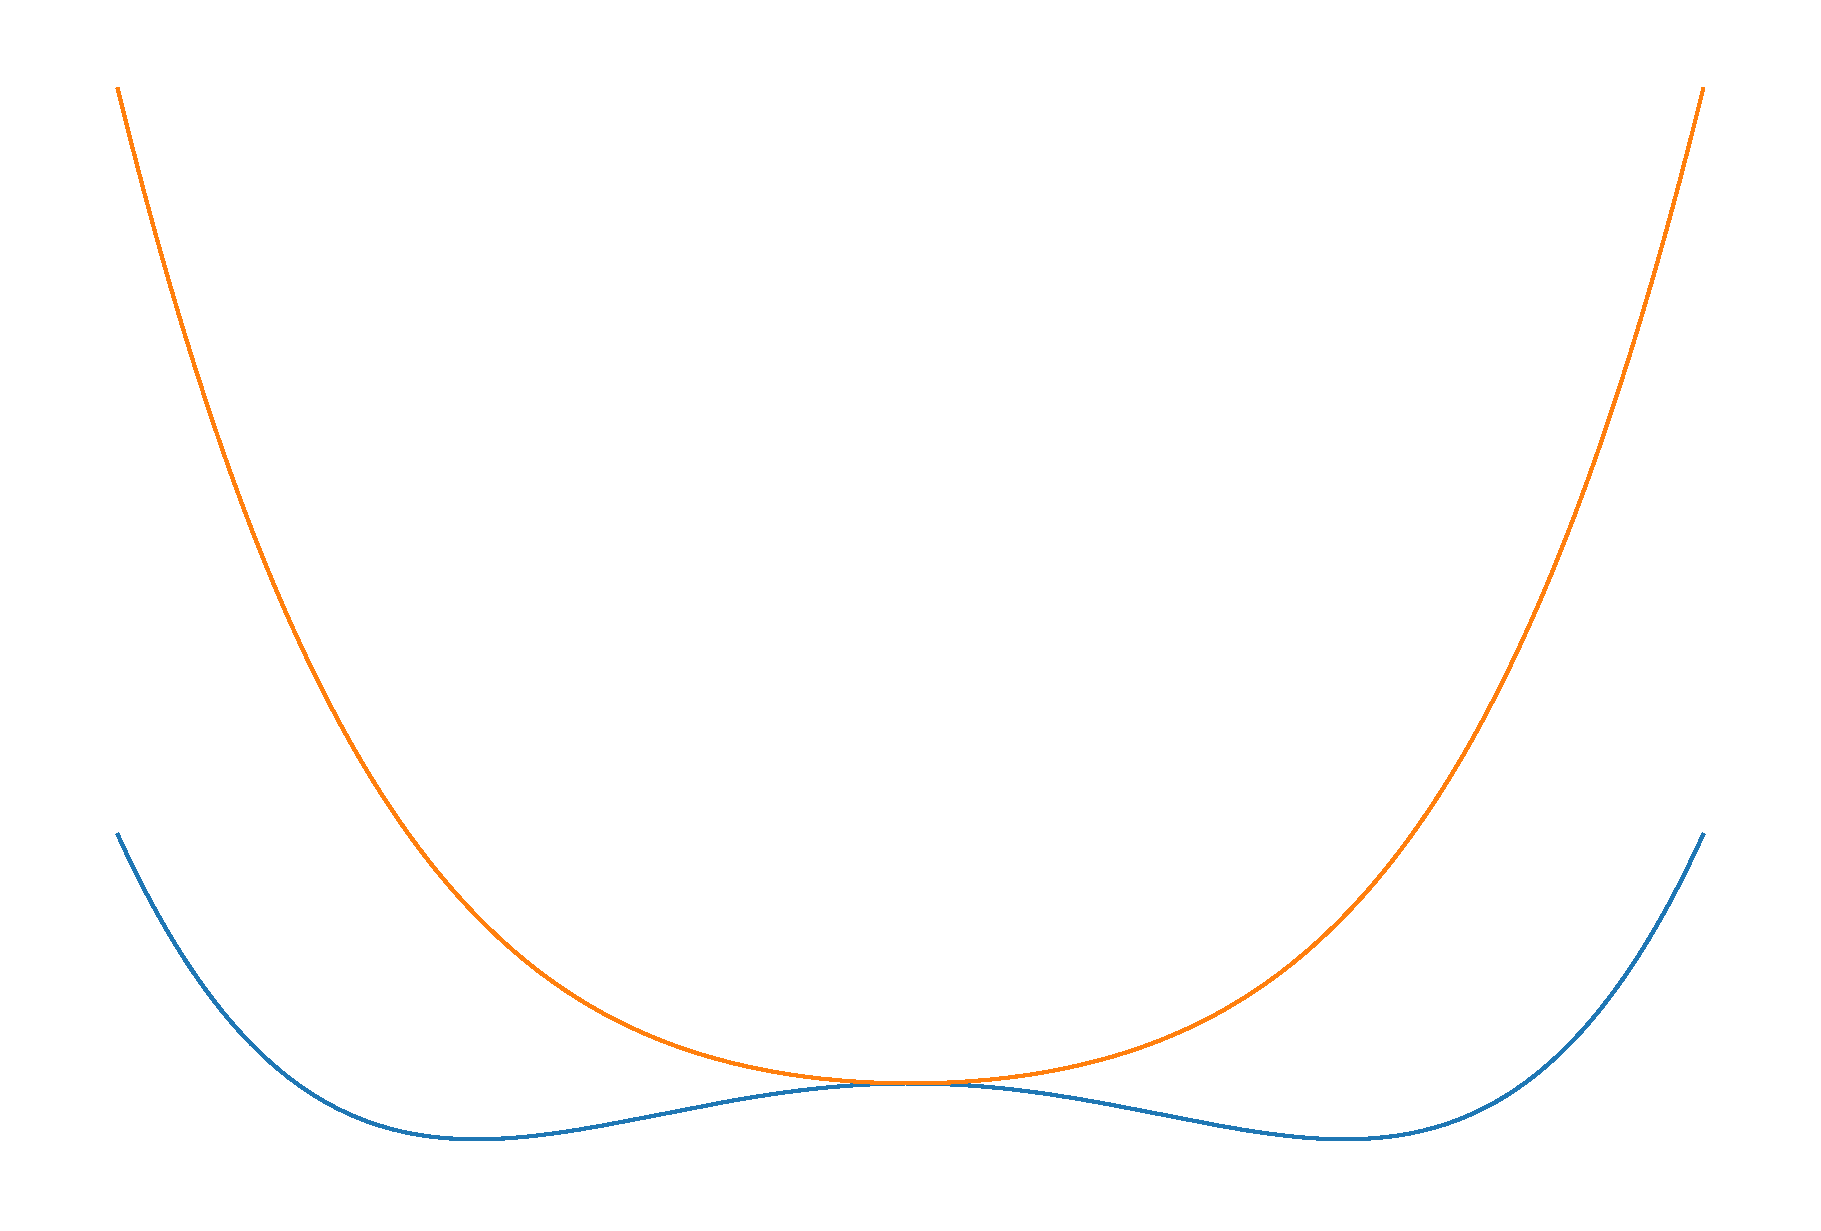
\includegraphics[width=0.6\linewidth]{./rSSB/rSSB.eps}
   \caption{SSB for real scalar field}%
   \label{fig:rSSB}
\end{figure}

We choose the vacuum state to be $+v$. Split the field into two parts (it makes the physics and observable more obvious), the vacuum $v$ and perturbation around the vacuum $\eta$
\begin{align*}
   \phi(x) &= v + \eta(x) \\
   v &= \expval{\phi} = \sqrt{\frac{-\mu^2}{\lambda}} = \text{const} \\
   \expval{\eta (x)} &= 0 \\
   \partial_\mu \phi &= \partial_\mu \eta 
\end{align*}

The kinetic term turns into
\begin{align*}
   (\partial_\mu \phi)(\partial^\mu \phi) &=  (\partial_\mu \eta)(\partial^\mu \eta) \\
   V &= \frac{1}{2}\mu^2 (v+\eta)^2 + \frac{1}{4} \lambda (v+\eta)^4 \\
     &= \frac{1}{2} \mu^2 v^2 + \frac{1}{2} \mu^2 \eta^2 + \mu^2 v\eta + \frac{1}{4} \lambda \left[ v^4 + 4 v^3 \eta + 6 v^2 \eta^2 + 4 v \eta^3 + \eta^4 \right] \\
     &= \frac{1}{2} \mu^2 v^2 + \frac{1}{4} \lambda v^2 + \eta \left(\mu^2 v + \lambda v^3 \right) + \eta^2 \left(\frac{1}{2}\mu^2+ \frac{6}{4} v^2 \lambda \right) + \lambda v \eta^3 + \frac{1}{4} \lambda \eta^4 \\
   \shortintertext{since $v = \sqrt{-\mu^2/\lambda}$, $\mu^2 v + \lambda v^3 = v (\mu^2 + \lambda v^2)=0$. There is no longer mirror symmetry in $\eta$. Now the mass is}
   \eval{\frac{\partial^2 V}{\partial \eta^2}}_{\eta=0} &= \mu^2 + 3v^2 \lambda = \mu^2 + 3 \left(\frac{-\mu^2}{\lambda} \right)\lambda = -2\mu^2
   \shortintertext{thus}
m_\eta &= \sqrt{-2\mu^2}
\end{align*}

After symmetry breaking $V(\eta)$ contains $\eta^3$ and $\eta^4$ terms, thus additional Feynman rules.
\begin{align}
   \feynmandiagram[small, horizontal=a to x, inline=(x.base)]{
      a --[scalar] x[dot] --[scalar] {b, c},
   };
   &\sim \lambda v \\
   \feynmandiagram[small, horizontal=a to b, inline=(x.base)]{
      {a,d} --[scalar] x[dot] --[scalar] {b, c},
   };
   &\sim \frac{1}{4} v
\end{align}

%%%%%%%%%%%%%%%%%%%%%%%%%%%%%%%%%%%%%%%%%%%%%%%%%%%%%%%%%%%%%%%%%
% Lecture date: 19-11-04
%%%%%%%%%%%%%%%%%%%%%%%%%%%%%%%%%%%%%%%%%%%%%%%%%%%%%%%%%%%%%%%%%

\subsection{Complex Field}
Now we want to consider complex scalar field $\phi(x) \in \Co$. We can also write the fields as
\begin{align}
   \phi(x) = \frac{1}{\sqrt{2}} \left( \phi_1(x) + i\phi_2(x) \right)
\end{align}
with $\phi_1, \phi_2 \in \R$.

Only scalar fields can get a vacuum expectation value, otherwise it violates Lorentz invariance. Vacuum has spin and then constantly interacts with all particles. 

The Lagrangian must be real, $\lag \in \R$
\begin{align}
   \lag = ( \partial_\mu \phi^* ) ( \partial^\mu \phi ) - \mu^2 \phi^* \phi - \lambda (\phi^* \phi)^2
\end{align}
This is invariant under transformation $\phi(x) \mapsto \euler^{i\alpha} \phi(x), \alpha \in \R$. Rewrite the Lagrangian with $\phi_1$ and $\phi_2$
\begin{align*}
   \lag =  \left( \partial_\mu \phi_1 \right) \left( \partial^\mu \phi_1 \right) + \left( \partial_\mu \phi_2 \right) \left( \partial^\mu \phi_2 \right) - \frac{1}{2} \mu^2 (\phi_1^2 + \phi_2^2) - \frac{1}{4} \lambda (\phi_1^2 + \phi_2^2)^2
\end{align*}
The last two terms are $-V(\phi)$

\begin{itemize}
   \item $\mu^2 > 0$. Minimum is at $\phi_1 = \phi_2 = 0$
   \item $\mu^2 < 0$. The potential has the shape of Mexican hat.
   \begin{figure}[htpb]
      \centering
      \includegraphics[width=0.4\linewidth]{cSSB/mh.pdf}
      \caption{Mexican hat\cite{wikiSSB}}%
      \label{fig:mexicanHat}
   \end{figure}
      We have set of minima forming a circular line $\phi_1^2 + \phi_2^2 = v^2 = -{\mu^2}/{\lambda}$. As an example $\phi_1 = v$ and $\phi_2 = 0$ and $\Uni(1)$ symmetry is spontaneous broken. The choice of vacuum breaks symmetry spontaneously.
      Field shift
      \begin{align}
         \phi(x) = \frac{1}{\sqrt{2}} \Big[ \underbrace{v + \eta(x)}_{\phi_1} + i \underbrace{\xi(x)}_{\phi_2} \Big]
      \end{align}
      with $\eta(x), \xi(x) \in \R$ and $\expval{\eta} = \expval{\xi}=0$.
      Insert into $V(\phi) = V(\phi_1, \phi_2)$
      \begin{align}
         \lag(\eta, \xi) = \frac{1}{2} (\partial_\mu \xi) (\partial^\mu \xi) + \frac{1}{2} (\partial_\mu \eta) (\partial^\mu \eta) + \text{const} + \mu^2 \eta^2 + (\text{cubic and quartic in $\eta$, $\xi$})
      \end{align}
      so $m_\eta^2 = -2\mu^2$ but $m_\xi^2 = 0$
\end{itemize}
Continuous global symmetry is spontaneously broken and it leads to massless state. It is called \underline{Goldstone theorem}. The massless state is the Goldstone boson.

\subsection{Higgs Mechanism}
Modify the transformation to
   \begin{align*}
   \phi(x) \mapsto \euler^{i\alpha(x)} \phi(x)
\end{align*}
with $\phi(x) \in \Co$ and $\alpha(x) \in \R$.

First step is to extend $\lag_\phi$ such that is invariant under this transformation. Introduce a spin-$1$ field $A_\mu(x)$ with the covariant derivative
\begin{align*}
   D_\mu &= \partial_\mu - ieA_\mu \\
   A_\mu &\mapsto A_\mu + \frac{1}{e} \partial_\mu \alpha
\end{align*}
The new Lagrangian
\begin{align}
   \lag = (D_\mu \phi)^* (D^\mu \phi) - \mu^2 \phi^* \phi - \lambda (\phi^* \phi)^2 - \frac{1}{4} F^{\mu\nu}F_{\mu\nu}
\end{align}
with $F_{\mu\nu}=\partial_\mu A_\nu - \partial_\nu A_\mu$. It contains the interaction between two $\phi$ and two $A_\mu$ \feynmandiagram[small, layered layout, inline=(x.base)]{a --[scalar] x --[scalar] b, c -- [photon]x--[photon]d,};

% $\mu^2 < 0, \phi = \frac{1}{\sqrt{2}}(v + \eta + i \xi)$

%%%%%%%%%%%%%%%%%%%%%%%%%%%%%%%%%%%%%%%%%%%%%%%%%%%%%%%%%%%%%%%%%
% Lecture date: 19-11-05
%%%%%%%%%%%%%%%%%%%%%%%%%%%%%%%%%%%%%%%%%%%%%%%%%%%%%%%%%%%%%%%%%

We want to look at spontaneous symmetry breaking of this system. We still want $\lambda > 0$, bound from below. In the case of $\mu^2 > 0$, symmetry not broken and we have scalar QED. In particle physics we do have charged scalars, such as $\pi^{\pm}$, $K^{\pm}$ and so on. We need $\mu^2 < 0$ to have spontaneous symmetry breaking. The field shift is as before
\begin{align}
   \phi(x) &= \frac{1}{\sqrt{2}} \left( v + \eta (x) + i \xi (x) \right) \\
   \begin{split}
   \lag(\eta, \xi) &= \frac{1}{2} (\partial_\mu \xi) (\partial^\mu \xi) + \frac{1}{2} (\partial_\mu \eta) (\partial^\mu \eta) - \lambda v^2 \eta^2 + \frac{1}{2} e^2 v^2 A_\mu A^\mu \\ 
                   &\quad - ev A_\mu \partial^\mu \xi - \frac{1}{4}F_{\mu\nu}F^{\mu\nu}  + (\text{scalar interaction temrs})
   \end{split}
\end{align}
So $m_\eta = \sqrt{2\lambda v^2}$, $m_A = ev$ and $m_\xi = 0$.

$A_\mu \partial^\mu \xi$ seems to mix $A$ and $\xi$. Massless spin $1$ has two degrees of freedom. $A_\mu(x)$ has four components, but Lorentz and gauge invariance restrict to two. Photon has two polarizations. Massive spin $1$ has three degree of freedom. We will show later on, $\xi$ is actually the additional degree of freedom of $A$. The term $A_\mu A^\mu$ breaks the gauge invariance.

To see physics, the choice of $\eta$ and $\xi$ is not very good. Instead choose
\begin{align}
   \phi \mapsto \frac{1}{\sqrt{2}} \left( v + h(x) \right) \euler^{i {\Theta(x)}/{v}}
\end{align}
with $h(x) \in \R, \Theta(x) \in \R$. We interpret this as a gauge transformation with $\alpha={\Theta} /  v$. To rewrite gauge transformation of $A_\mu(x)$
\begin{align}
   A_\mu \mapsto A_\mu + \frac{1}{ev}\partial_\mu \Theta(x)
\end{align}

The Lagrangian becomes
\begin{align}
   \lag = \frac{1}{2} (\partial h)^2 - \lambda v^2 h^2 + \frac{1}{2} e^2 v^2 A_\mu A^\mu - \lambda v h^3 - \frac{1}{4} \lambda h^4 + \frac{1}{2} e^2 A^2 h^2 -\frac{1}{4} F_{\mu\nu}F^{\mu\nu}
\end{align}
$\xi$ is no longer there. This is \underline{Higgs mechanism}. So we have before $2+2$ degree of freedom ($\eta$, $\xi$, $A^{m=0}$) to $1+3$ degrees of freedom ($h$, $A^{m \neq 0}$).

Phase transition in magnetism is an example of symmetry breaking. Magnetization is temperature dependent. In the early universe the temperature is high so that $\mu^2(T) > 0$. As it cools down $\mu^2 < 0$.

\subsection{Spontaneous Breaking of local $\SU(2)$ Theory}
We start with ungauged, complex scalar field
\begin{align}
   \lag &= (\partial_\mu \phi)^\dagger (\partial^\mu \phi) - \mu^2 \phi^\dagger \phi -\lambda (\phi^\dagger \phi)^2
   \shortintertext{Now $\phi$ contains two complex scalar fields.}
   \phi &= \begin{pmatrix} \phi_\alpha \\ \phi_\beta \end{pmatrix} = \frac{1}{\sqrt{2}} \begin{pmatrix} \phi_1 + i\phi_2 \\ \phi_3 + i\phi_4 \end{pmatrix}
\end{align}
with $\phi_{1,2,3,4} \in \R$.

Gauge transformation
\begin{align}
   \phi \mapsto \phi'=\euler^{i\alpha_a(x) \tau_a / 2} \phi
\end{align}
There are only three generators of $\SU(2)$, $a=1,2,3$.

Introduce three gauge bosons $W_\mu^a$, $a=1,2,3$. Define the covariant derivative
\begin{align}
   D_\mu = \partial_\mu - ig \frac{\tau_a}{2} W_\mu^a
\end{align}
Note $T^a = {\tau^a} / {2}$.

The $\tau$ matrices are Pauli matrices
\begin{align}
   \tau_3 = \begin{pmatrix} 1 & 0 \\ 0 & -1\end{pmatrix}   \quad 
   \tau_2 = \begin{pmatrix} 0 & -i \\ i & 0\end{pmatrix} \quad
   \tau_1  = \begin{pmatrix} 0 & 1 \\ 1 & 0\end{pmatrix} 
\end{align}

Have gauge transformation of $W_a^\mu$
\begin{align}
W_\mu^a \mapsto W_\mu^a - \frac{1}{g} \partial_\mu \alpha^a - f^{abc} \alpha_b W_{c \,\mu} 
\end{align}
Here $f_{abc} = \epsilon_{abc}$ totally symmetric tensor in three dimension.

Lagrangian becomes
\begin{align}
   \lag &= (D_\mu \phi)^\dagger (D^\mu \phi) - V(\phi) - \frac{1}{4} W_{\mu\nu}^a W^{a \, \mu\nu} \\
   \shortintertext{Kinetic term for gauge fields}
   W_{\mu\nu}^a &= \partial_\mu W_\nu^a - \partial_\nu W_\mu^a - g (W_\mu \times W_\nu)^a \\
   \shortintertext{The potential}
   V(\phi) &= \mu^2 \phi^\dagger \phi + \lambda (\phi^\dagger \phi)^2
\end{align}

We are interested in the case $\lambda > 0$ and $\mu^2 < 0$. Minima are at
\begin{align*}
   \phi^\dagger \phi = \frac{1}{2} \left( \phi_1^2 + \phi_2^2 + \phi_3^2 + \phi_4^2 \right) = - \frac{\mu^2}{2\lambda}
\end{align*}
We can make a choice for minimum $\phi_1 = \phi_2 = \phi_4 = 0$ and $\phi_3^2 = v^2 = - {\mu^2}/{\lambda}$ 
\begin{align}
   \expval{\phi} = \frac{1}{\sqrt{2}} \begin{pmatrix} 0 \\ v\end{pmatrix}
\end{align}
with $v \in \R$.

Shift of $\phi$ field
\begin{align}
   \phi(x) &\mapsto \euler^{i \hat{\tau} \cdot \hat{\theta} / v} \phi(x) = \euler^{i \hat{\tau} \cdot \hat{\theta} / v} \frac{1}{\sqrt{2}}  \begin{pmatrix} 0 \\ {v +h(x)} \end{pmatrix}
\end{align}

Infinitesimal expansion in $\theta(x)$
\begin{align*}
   \phi(x) &= \frac{1}{\sqrt{2}} \left( \id + i \hat{\tau} \cdot \hat{\theta}(x)/v \right) \begin{pmatrix} 0 \\ {v + h(x)}\end{pmatrix} \\
&= \frac{1}{\sqrt{2}} \begin{pmatrix} 1 + i\theta_3 /v & i(\theta_1 - i\theta_2)/v \\ i(\theta_1 + i\theta_2) / v & 1 - i\theta_3 /v \end{pmatrix} \begin{pmatrix} 0 \\ v + k(x)\end{pmatrix}
\end{align*}

Look at kinetic term in $\phi$
\begin{align*}
   \lag_{\text{kin}}^\phi &= (D_\mu \phi)^\dagger (D^\mu \phi) \\
                          &= \left( \partial_\mu \phi + i g \hat{\tau} \cdot \hat{W} \phi \right)^\dagger \left( \partial^\mu \phi + i g \hat{\tau} \cdot \hat{W} \phi \right) \\
                          \shortintertext{compute at minimum $\phi = \frac{1}{\sqrt{2}} \begin{pmatrix} 0 \\ v\end{pmatrix}$}
                          \left| \frac{i}{2} g \hat{\tau} \cdot \hat{W} \phi \right|^2 & = \frac{g^2}{8}a \left| \begin{pmatrix} W^3_\mu & W^1_\mu - i W_\mu^2 \\ W^1_\mu + i W_\mu^2 & -W_\mu^3 \end{pmatrix} \begin{pmatrix} 0 \\ v\end{pmatrix} \right|^2 \\
                         &= \frac{g^2 v^2}{8} \left| \begin{pmatrix} W_\mu^1 - iW_\mu^2 \\ -W_\mu^3\end{pmatrix} \right|^2 \\
                         &= \frac{g^2 v^2}{8} \pmb{W}^2 \\
                         &= \frac{1}{2} M^2 \pmb{W}^2
\end{align*}
with $M = gv/2$. We spontaneously broken $\SU(2)$ gauge theory. However, this is not realized in nature.
